\section{\textit{Double Dispatch}}
  Idealmente queremos que el daño que un \textit{Bakémon} hace a otro dependa de su tipo y el tipo 
  del \textit{Bakémon} atacado, pero también nos gustaría una forma de hacer la comprobación de 
  tipos sin tener que preguntar por el tipo de cada \textit{Bakémon} en cada ataque.

  Nos gustaría poder hacer algo como:

  \begin{kotlin}
    interface Bakemon {
      val name: String
      var health: Int
      val level: Int
      val attack: Int

      fun attackBakemon(bakemon: FireBakemon)
      fun attackBakemon(bakemon: WaterBakemon)
      fun attackBakemon(bakemon: GrassBakemon)
      fun takeDamage(damage: Int)
    }
  \end{kotlin}

  \begin{kotlin}
    class FireBakemon(name: String, health: Int, level: Int, attack: Int) :
        AbstractBakemon(name, health, level, attack) {
      override fun attackBakemon(bakemon: FireBakemon) = bakemon.takeDamage(attack / 2)
      override fun attackBakemon(bakemon: WaterBakemon) = 
        bakemon.takeDamage((attack * 1.5).toInt())
      override fun attackBakemon(bakemon: GrassBakemon) = bakemon.takeDamage(attack)
      ...
    }
  \end{kotlin}

  Pero si intentamos ejecutar esto obtendremos un error de compilación en la función
  \mintinline{kotlin}{`Bakemon can attack Bakemon`} (\cref{fig:ambiguous-call-error}) porque
  no existe una función \mintinline{kotlin}{attackBakemon(Bakemon)}.
  Podemos agregar esa función, pero entonces cada vez que hagamos \mintinline{kotlin}{attackBakemon}
  estaremos llamando al método \mintinline{kotlin}|attackBakemon(Bakemon)| ya que \texttt{Bakemon}
  es supertipo de \texttt{FireBakemon}, \texttt{WaterBakemon} y \texttt{GrassBakemon}.

  \begin{figure}[ht!]
    \centering
    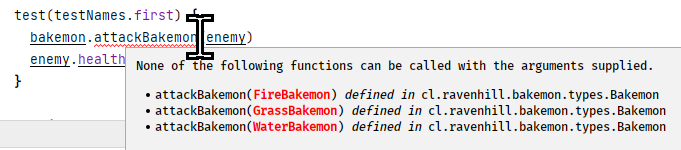
\includegraphics[width=0.8\textwidth]{img/oop/dd/ambiguous-call-error.png}
    \caption{Error de compilación por ambigüedad}
    \label{fig:ambiguous-call-error}
  \end{figure}

  El proceso mediante el que se resuelve el método a llamar se llama \textit{enlace dinámico} 
  (\textit{dynamic dispatch}).
  En el enlace dinámico, el compilador no puede saber qué método se va a llamar hasta que se ejecute
  el programa.
  Aquí entra en juego el concepto de \textit{ambigüedad}.
  
  Existen dos tipos de enlace dinámico: \textit{single dispatch} y \textit{multiple dispatch}.
  
  En \textit{single dispatch} el programa decide qué método llamar basándose en el tipo de la
  instancia sobre la que se llama al método.
  Es decir, se decide qué método llamar basándose en un sólo parámetro.
  Volvamos al ejemplo de la familia \textit{Caninae} del \cref{chap:oop2} y veamos cómo se resuelve
  el enlace dinámico de la funcionalidad de mover la cola.

  \begin{kotlin}
    interface Canine {
      fun wagTail()
    }
  \end{kotlin}

  \begin{kotlin}
    class Wolf : Canine {
      override fun wagTail() = println("Wolf wagging tail")
    }
  \end{kotlin}

  \begin{kotlin}
    class Dog : Canine {
      override fun wagTail() = println("Dog wagging tail")
    }
  \end{kotlin}

  \begin{kotlin}
    class Fox : Canine {
      override fun wagTail() = println("Fox wagging tail")
    }
  \end{kotlin}

  \begin{kotlin}
    fun main() {
      val wolf = Wolf()
      val dog = Dog()
      val fox = Fox()
      wolf.wagTail()
      dog.wagTail()
      fox.wagTail()
    }
  \end{kotlin}

  En estos casos, el compilador sabe que el tipo de la instancia sobre la que se llama al método
  \mintinline{kotlin}{wagTail()} es \texttt{Wolf}, \texttt{Dog} o \texttt{Fox} respectivamente.
  Al objeto que recibe el mensaje lo llamamos \textit{receptor} del mensaje.
  En este caso, los receptores son \texttt{wolf}, \texttt{dog} y \texttt{fox}.
  Entonces, la decisión de qué método llamar se basa en el tipo del receptor.

  En \textit{multiple dispatch} el programa decide qué método llamar basándose en el tipo de la
  instancia sobre la que se llama al método y en los tipos de las instancias que se pasan como
  argumentos.
  Es decir, se decide qué método llamar basándose en dos o más parámetros.
  En el ejemplo de los \textit{Bakémon} queremos que el daño que un \textit{Bakémon} hace a otro
  dependa de su tipo y el tipo del \textit{Bakémon} atacado.
  
  Entonces lo que nos gustaría hacer en nuestro programa es \textit{multiple dispatch}.
  El problema es que \textit{Kotlin} (y la mayoría de los lenguajes) no soporta \textit{multiple
  dispatch}.
  ¿Cómo podemos hacer entonces para que el daño que un \textit{Bakémon} hace a otro dependa de su
  tipo y el tipo del \textit{Bakémon} atacado?
  La solución es usar \textit{double dispatch}.

  \begin{defaultbox}[Double Dispatch]
    \index{Double Dispatch}

    \textit{Double dispatch} es un mecanismo que permite implementar \textit{multiple dispatch} en
    lenguajes que no lo soportan.
    
    En \textit{double dispatch} se realizan dos llamados a métodos (\textit{single dispatch}):
    \begin{itemize}
      \item El primer llamado desambigua el tipo del receptor del mensaje.
      \item El segundo llamado desambigua el tipo del argumento del mensaje.
    \end{itemize}
  \end{defaultbox}

  Veamos esto con un ejemplo.
  El \textit{cachipún} (piedra, papel o tijera) es un juego de manos en el que cada jugador
  simultáneamente muestra una de las tres posibilidades formando así un triángulo.
  El jugador que muestra la opción que gana es el ganador de la ronda.
  Las posibilidades son:

  \begin{itemize}
    \item Piedra gana a tijera.
    \item Tijera gana a papel.
    \item Papel gana a piedra.
  \end{itemize}

  Modelemos este juego con \textit{Kotlin} usando \textit{double dispatch}.

  Lo primero que necesitaremos es una interfaz que abarque a las tres opciones del juego.

  \begin{kotlin}
    interface Hand {
      fun playWith(hand: Hand)
      ...
    }
  \end{kotlin}

  Ahora definamos las tres opciones del juego.

  \begin{kotlin}
    class Rock : Hand {
      override fun playWith(hand: Hand) = hand.playWithRock(this)
      ...
    }
  \end{kotlin}

  Veamos lo que pasa cuando llamamos al método \mintinline{kotlin}{playWith(hand: Hand)} con un
  \texttt{Rock} como receptor y un \texttt{Paper} como argumento.
  Lo primero que hace el compilador es desambiguar el tipo del receptor del mensaje.
  Como el receptor es un \texttt{Rock}, el compilador sabe que debe llamar al método
  \mintinline{kotlin}|Rock::playWith(Hand)|.
  Luego, el receptor del segundo mensaje es el \texttt{Paper} que se pasa como argumento, así que
  el programa sabe que debe llamar al método \mintinline{kotlin}|Paper::playWithRock(Rock)|.

  Por último podemos definir el método \mintinline{kotlin}|Hand::playWithRock(Rock)|.

  \begin{kotlin}
    interface Hand {
      fun playWithRock(rock: Rock)
      ...
    }
  \end{kotlin}

  \begin{kotlin}
    class Paper : Hand {
      override fun playWithRock(rock: Rock) = println("Paper wins")
      ...
    }
  \end{kotlin}